\documentclass[11pt,a4paper]{article}
\usepackage[utf8]{inputenc}
\usepackage[spanish]{babel}
\usepackage{amsmath}
\usepackage{amsfonts}
\usepackage{amssymb}
\usepackage{graphicx}
\usepackage[left=2cm,right=2cm,top=2cm,bottom=2cm]{geometry}
\author{Valdez Bernal Maria Fernanda\\Valdez Esquivel Melani Betsabee\\
González Pardo Adrian}

\title{Reporte de practica 1}
\newcommand\tab[1][1cm]{\hspace*{#1}}
\begin{document}
\maketitle
\section{Introducción}
La problematica principal de la practica es que a traves del uso de hilos y de programación "paralela" podamos leer $M \geq 20$ archivos de cualquier extensión (se selecciono la extensión .txt), en los cuales a traves de una cantidad $N$ hilos, donde matemáticamente deben cumplir la condición de $N \leq M$, por lo que en el programa se debe validar que no haya más hilos que archivos.
\section{Desarrollo}
Para la realización del programa primeramente se tomaron algunas ideas acerca de los ejercicios de hilos hechos previamente en la clase, algunos de ellos es saber como planificar que $N$ cantidad de hilos le corresponda trabajar con al menos $1$ archivo dependiendo la planificación que se realizara y se ilustrara en el diagrama de flujo. Por ello a groso modo la resolución de problema sera realizada bajo el lenguaje C y la realización de este tipo de tareas sera con llamadas de procesos $popen$ en el cual abre flujos de entrada/salida, en los cuales nos permitiran hacer llamadas de algunos comandos que nos puede proporcionar el Sistema Operativo (OS / SO), para la lectura y llenado de buffer, por otro lado tambien gracias a este tipo de llamadas podemos hacer que las tareas de lectura de cada archivo pase por medio de tuberías (Pipes) el buffer de salida para la eliminación de caracteres no solicitados, así como la separacion de cadenas de caracteres extensas que pueden formar renglones u oraciones y poderlas separar por cada palabra contenida en el archivo aún cuando estas se repitan.
\subsection{Diagrama de flujo}
\begin{center}
  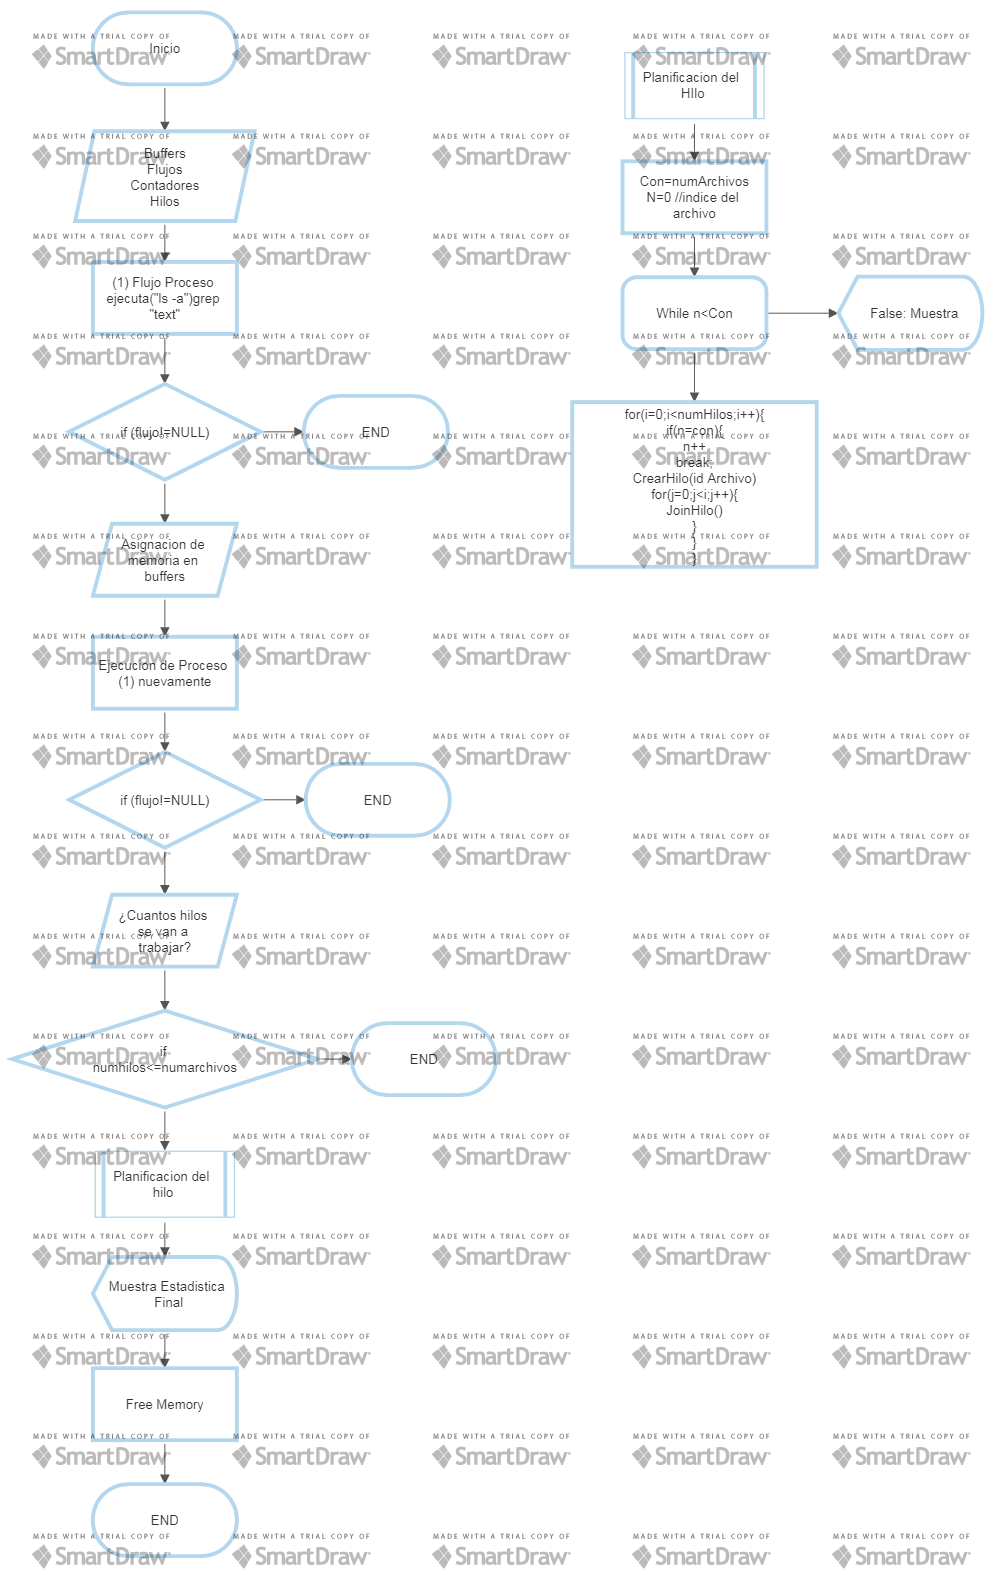
\includegraphics[scale=0.4]{diagramaFlujo.png}\\
  \textit{Figura 1: descripción a groso modo de lo que hay en main sin usar llegar aun a la parte del hilo}
  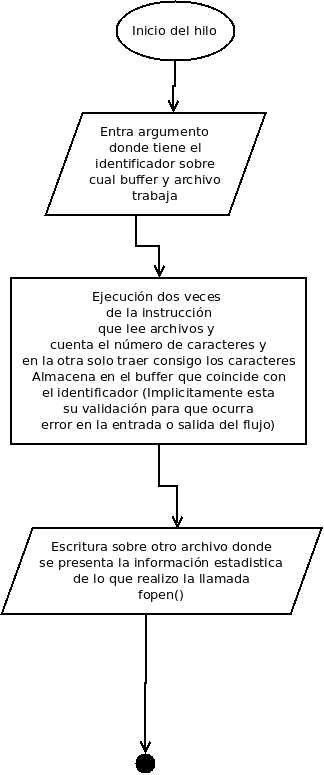
\includegraphics[scale=0.5]{diagramaHilo.png}\\
  \textit{Figura 2: descripción a groso modo de las tareas que realiza el hilo}
\end{center}
\subsection{Explicación del diagrama de flujo}
\begin{itemize}
  \item En la $figura$ $1$ podemos observar descriptivamente el uso de variables y el como lógicamente trabajara la aplicación, si bien por un lado vemos dos una aproximación a como se realiza la llamada a la subrutina de la $figura$ $2$, tambien se explica a groso modo el como se valida el numero de hilos y el tipo de llamada a popen para el conteo de los archivos existentes en el directorio, así como la tarea de la planificación de como sera repartida la carga de trabajo.
  \item En la $figura$ $2$ podemos observar de forma explicativa lo que realiza el hilo, por lo que indirectamente y sin necesidad de extendernos demasiado con su explicación la tarea que realiza es generar una estadística donde en un archivo de extensión .csv se puede guardar las palabras y en numero de apariciones que tienen en cada archivo de texto así como resguardar en las variables datos que nos permitiran regresar a la rutina donde esta la función main.
\end{itemize}

\section{Conclusiones}
\subsection{Valdez Bernal Maria Fernanda}
Para trabajar eficientemente esta práctica, el uso de hilos en la lectura de archivos, juega un papel muy importante puesto que los procesos que se ejecutan en ellos, dividen el trabajo para obtener un mejor rendimiento en conjunto con los identificadores, los cuales, nos permitieron tomar el control sobre cada archivo.\\
Para la implementación de esta práctica, de entre todas las formas de comunicación de procesos, se decidió usar la herramienta de tuberías por que permiten entablar una conexión más eficiente para la transmisión de datos entre los hilos padres e hijos. Y en relación a esto, la búsqueda de palabras y el conteo, fue fácilmente resuelta dado que implementamos este tipo de técnicas, tanto para escribir en los buffers de entrada como los de salida.
\subsection{Valdez Esquivel Melani Betsabee}
El uso de hilos nos facilito mucho el manejo de los archivos para poder hacer mas eficiente el proceso, ya que haciendolo de manera tradicional de archivo por archivo era mas tardado para el programa
, tambien para hacer el estdistico de las palabras nos fue muy util el uso de los hilos, ya que cada hilo puede manejar y guardar informacion de un archivo o mas sin afectar la informacion de
algun otro hilo.\\
Tambien combinar lo que son las tuberias para hacer un estilo de sincronizacion para no perder lo que es la secuencia de la informacion.
\subsection{González Pardo Adrian}
Las llamadas con uso de flujos de entrada/salida de FILE nos permite tanto manejar el flujo de archivos para lectura y escritura, así como llamadas de procesos externos que puede realizar un terminal de Linux, nos permitío el trabajar con los identificadores de los hilos así como llevar un control sobre el identificador del archivo y realizar todas las tareas de retornar alguna escritura sobre archivo o sobre algun buffer del programa, el realizar el conteo de palabras fue sencillo gracias a que se realizo la busquedad de las llamadas, donde permiten limpiar el buffer de salida del archivo eliminando espacios y algunos caracteres que pueden ser no necesarios en la realización de la tarea.






\end{document}
